\documentclass[10pt,a4paper]{amsart}
\usepackage[margin=19mm]{geometry}
\usepackage{amsmath,amssymb,mathtools}
\usepackage[scr=rsfs,cal=euler]{mathalfa}
\usepackage{xfrac}
\usepackage[unicode,hidelinks,bookmarks=false]{hyperref}
\newcommand{\ie}{i.e.\ }
\newcommand{\cf}{cf.\ }
\newcommand{\resp}{respectively\ }
\newcommand{\Subsection}{\subsection}
\providecommand{\nobreakdash}{\nobreak\hbox{-}}
\setlength{\emergencystretch}{2em}
\multlinegap0pt
\usepackage{tikz}
\usepackage{float}
\usepackage{mathtools}
\usepackage{amssymb}
\usepackage{caption}
\usepackage{enumerate}
\usepackage[all]{xy}
\usepackage{csquotes}
\newtheorem{theorem}{Theorem}
\newtheorem{example}{Example}
\newtheorem{lemma}{Lemma}
\newtheorem{corollary}{Corollary}
\newcommand{\FN}[1]{$\textbf{F}_{#1}$}
\title{Tree Pairs for Algebraic Bieri-Strebel Groups}
\author{Lewis Molyneux}
\date{Source: arXiv:2602.08748v1 (CC BY 4.0)}
\begin{document}
\maketitle

\noindent\emph{Source and licence.} Tree Pairs for Algebraic Bieri-Strebel Groups. Version arXiv:2602.08748v1 (CC BY 4.0), distributed by arXiv under the Creative Commons Attribution 4.0 International licence, http://creativecommons.org/licenses/by/4.0/, as recorded in the arXiv licence metadata for this exact version and shown on the abstract page https://arxiv.org/abs/2602.08748v1. Full licence notice: \texttt{licenses/arxiv-2602.08748-CC-BY-4.0.txt}.\par\smallskip

\noindent\textit{Editorial scope.} Counted unit: the article's theorem roothm (source0.tex lines 624--626). The article's complete original proof of it is delivered with it (source0.tex lines 836--894, one \texttt{proof} environment of 59 lines, which the article places away from the statement). No mathematics is written, repaired or re-derived: the statement and the proof are the article's own lines, in the article's own notation, and no retained line is substituted or re-flowed.  Retained uncounted as the source-local context the proof needs: lines 631--639; lines 784--786; lines 815--817; lines 832--834.  Nothing was omitted from any retained span, so the package carries no omission record.  No retained line contains a citation, so the wrapper carries no bibliography and no bibliography entry.  The retained lines contain the article's own diagram code, which the wrapper typesets with the standard tikz packages; no image file is delivered and the package declares no asset dependency.  Editorial formatting only, in addition: an AMS \texttt{amsart} preamble that restates the article's own declarations and macros used by the retained lines, namely the environments \texttt{theorem}, \texttt{example}, \texttt{lemma}, \texttt{corollary} on separate counters, together with the standard packages those lines need.  The retained environments print in this document as Theorem 1, Example 1, Lemma 1, Corollary 1 in order of appearance, whereas the article prints the same items with the numbering of its own full document.  The complete native source of the article as distributed in the arXiv e-print for this exact version is bundled unchanged as \texttt{sources/194270/source0.tex}.
\begin{example} \label{rootfind}
For all $0<p \in \mathbb{Z}[\beta]$, where $\beta$ is the root of an $n$-th degree polynomial, is it possible to write:

$$
p = b_0 + b_1 \beta +...+b_{n_1} \beta^{n-1}
$$

where $b_i \in \mathbb{Z}_{\geq 0}$ for all $i$?
\end{example}

\begin{lemma}\label{rootexclude}
For any $\beta$ as the root of a quadratic subdivision polynomial $ax^2+bx-1$, $\sqrt{\beta}$ is not in $\mathbb{Z}[\beta]$.
\end{lemma}

\begin{corollary} \label{rootcor}
For any $\beta$ as the root of a quadratic subdivision polynomial $ax^2+bx-1$, $n \in \mathbb{N}$, $\sqrt[2n]{\beta}$ is not in $\mathbb{Z}[\beta]$.
\end{corollary}

\begin{lemma}\label{treepairdrop}
Consider $\beta$ as the unique positive root of $P(x) = a_n x^n +...+ a_1 x -1$ and $\sqrt[k]{\beta}$ as the root of $P(x^k) = a_n x^{kn} + ... + a_1 x^k -1$. Suppose the tree pair representation based of $P(x)$ is a well-defined tree pair representation for \FN{\beta}. Either \FN{\sqrt[k]{\beta}} $\cong$ \FN{\beta}, or the tree-pair based on $P(x^k)$ is not a well-defined tree-pair representation for \FN{\sqrt[k]{\beta}}. 
\end{lemma}

\begin{theorem}\label{roothm}
The Bieri-Strebel group with subdivision polynomial $ax^{2n}+bx^n-1$ cannot have a well defined tree-pair representation.
\end{theorem}

\begin{proof}[Proof of theorem \ref{roothm}]
To prove \ref{roothm}, we wish to construct an element we know is in \FN{\sqrt[2n]{\beta}} but cannot be in \FN{\beta}. We will construct an element that is in \FN{\sqrt{\beta}}, and by a similar argument to the proof of \ref{rootcor}, must be in \FN{\sqrt[2n]{\beta}} as well.
\par
We first create a partition pair which we know cannot be in \FN{\beta}. From \ref{rootexclude}, we know that if a partition pair contains $\sqrt{\beta}$ as a nontrivial breakpoint, then that partition pair cannot be an element of \FN{\beta}. From here, the simplest solution would be to have $\sqrt{\beta}$ as the sole breakpoint in the first partition and then have $1-\sqrt{\beta}$ as the sole breakpoint of the second partition. The issue with this is that the resulting map would map an interval of length $\sqrt{\beta}$ to an interval of length $1-\sqrt{\beta}$. This would require $\frac{1-\sqrt{\beta}}{\sqrt{\beta}}$ to be in $\langle \sqrt{\beta} \rangle$, which is challenging to prove. Instead, we will construct a partition pair that has only slopes in $\langle \beta \rangle$. Since $\langle \beta \rangle \subseteq \langle \sqrt{\beta} \rangle$, we can then guarantee our partition pair is in \FN{\sqrt{\beta}}.
\par
We create our partition pair in the following way. First we take two copies of the interval with $\sqrt{\beta}$ as the sole breakpoint. From here, we subdivide the interval of length $\sqrt{\beta}$ in each partition in different ways. Each interval will now be divided into $a$ intervals of length $\beta^2 * \sqrt{\beta}$ and $b$ intervals of length $\beta * \sqrt{\beta}$, where $\beta$ is the root of $ax^2+bx-1$, implying 

\begin{equation}
\begin{aligned}
a \beta^2 + b \beta & = 1 \\
a \beta^2 *\sqrt{\beta} + b \beta * \sqrt{\beta} & = \sqrt{\beta}
\end{aligned}
\end{equation}
\par
The ordering of the subintervals in the partitions is arbitrary, aside from 2 points. First, the sole interval of length $1-\sqrt{\beta}$ must be the $i$th interval in each partition for some $i$, and the partitions must not be identical. 

\begin{center}
\begin{figure}[H]
\centering
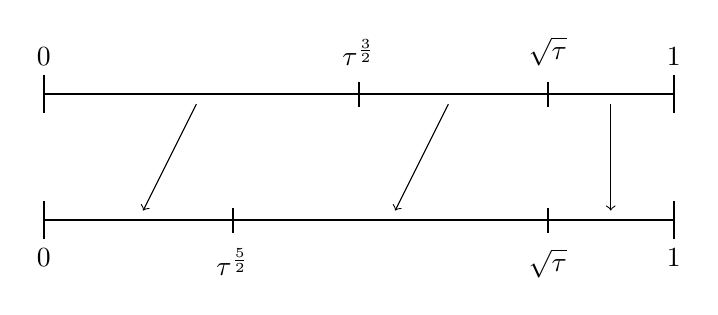
\begin{tikzpicture}[scale=8]
    \draw[thick] (1,0) -- (0,0);
    \draw[thick] (0,-0.2) -- (1, -0.2);
    \draw[thick] (0, 0.03) -- (0, -0.03);
    \draw[thick] (1,-0.03) -- (1, 0.03);
    \draw[thick] (0, -0.23) -- (0,-0.17);
    \draw[thick] (1, -0.23) -- (1, -0.17);
    \draw[thick] (0.8, 0.02) -- (0.8, -0.02);
    \draw[thick] (0.8, -0.22) -- (0.8, -0.18);
    \draw[thick] (0.5, 0.02) -- (0.5, -0.02);
    \draw[thick] (0.3, -0.22) -- (0.3, -0.18);
    \filldraw (0,0.03) circle (0pt) node[anchor=south]{$0$};
    \filldraw (1,0.03) circle (0pt) node[anchor=south]{$1$};
    \filldraw (0,-0.23) circle (0pt) node[anchor=north]{$0$};
    \filldraw (1,-0.23) circle (0pt) node[anchor=north]{$1$};
    \filldraw (0.8,-0.23) circle (0pt) node[anchor=north]{$\sqrt{\tau}$};
    \filldraw (0.8,0.03) circle (0pt) node[anchor=south]{$\sqrt{\tau}$};
    \filldraw (0.5,0.03) circle (0pt) node[anchor=south]{$\tau^{\frac{3}{2}}$};
    \filldraw (0.3,-0.23) circle (0pt) node[anchor=north]{$\tau^{\frac{5}{2}}$};
    \node (A) at (0.25,0) {};
    \node (B) at (0.65,0) {};
    \node (C) at (0.9,0) {};
    \node (D) at (0.15,-0.2) {};
    \node (E) at (0.55,-0.2) {};
    \node (F) at (0.9,-0.2) {};
    \draw[->](A)--(D);
    \draw[->](B)--(E);
    \draw[->](C)--(F);

\end{tikzpicture}
    
\caption{An example of a partition pair in \FN{\sqrt{\tau}} with the breakpoint $\sqrt{\tau}$ excluding it from \FN{\tau}. The slopes in this map have gradients $\tau$, $\tau^{-1}$ and $1$ from left to right}\label{roottau}
\end{figure}
\end{center}

As seen in the example \ref{roottau}, maps constructed in this way have gradients  in $\langle \sqrt{\beta} \rangle$ (indeed, they are in $\langle \beta \rangle$), but as they have $\sqrt{\beta}$ as a breakpoint, these maps are in \FN{\sqrt{\beta}} but not in \FN{\beta}. Thus, we can conclude that \FN{\beta} is not the same group as \FN{\sqrt{\beta}} and so the tree pair representation based on $P(x^2)$ is not a well-defined tree pair representation for \FN{\sqrt{\beta}} by \ref{treepairdrop}. Similarly, this element is in \FN{\sqrt[2n]{\beta}}, and so $P(x^{2n})$ is not a well-defined tree pair representation for \FN{\sqrt[2n]{\beta}}.
\par
Finally, we need to preclude the possibility of a different tree pair representation. For this we rely on our example to \ref{rootfind}. What we have shown with the example (and its generalisation) is that we can form an interval in a partition in \FN{\sqrt{\beta}} with a length that cannot be expressed in the form $a_4 \beta^{k+4} + a_3 \beta{k+3} + a_2 \beta^{k+2} + a_1 \beta^{k+1}$ via repeated subdivision (the substitution that multiplication by the matrix $A$ represents). However, were we constructing a tree to represent this partition, such an interval would have to be expressed in this way. As such, these intervals cannot be expressed as part of a tree pair presentation and thus we have our proof that Bieri-Strebel groups with associated polynomial $ax^4+bx^2-1$ cannot have a well defined tree-pair representation. Combining this with \ref{rootcor} is our proof of \ref{roothm}.

\end{proof}

\end{document}
